\section{Durchführung}
\label{sec:Durchführung}
Die komplette Messapparatur ist so aufgebaut:
\begin{figure}
\centering
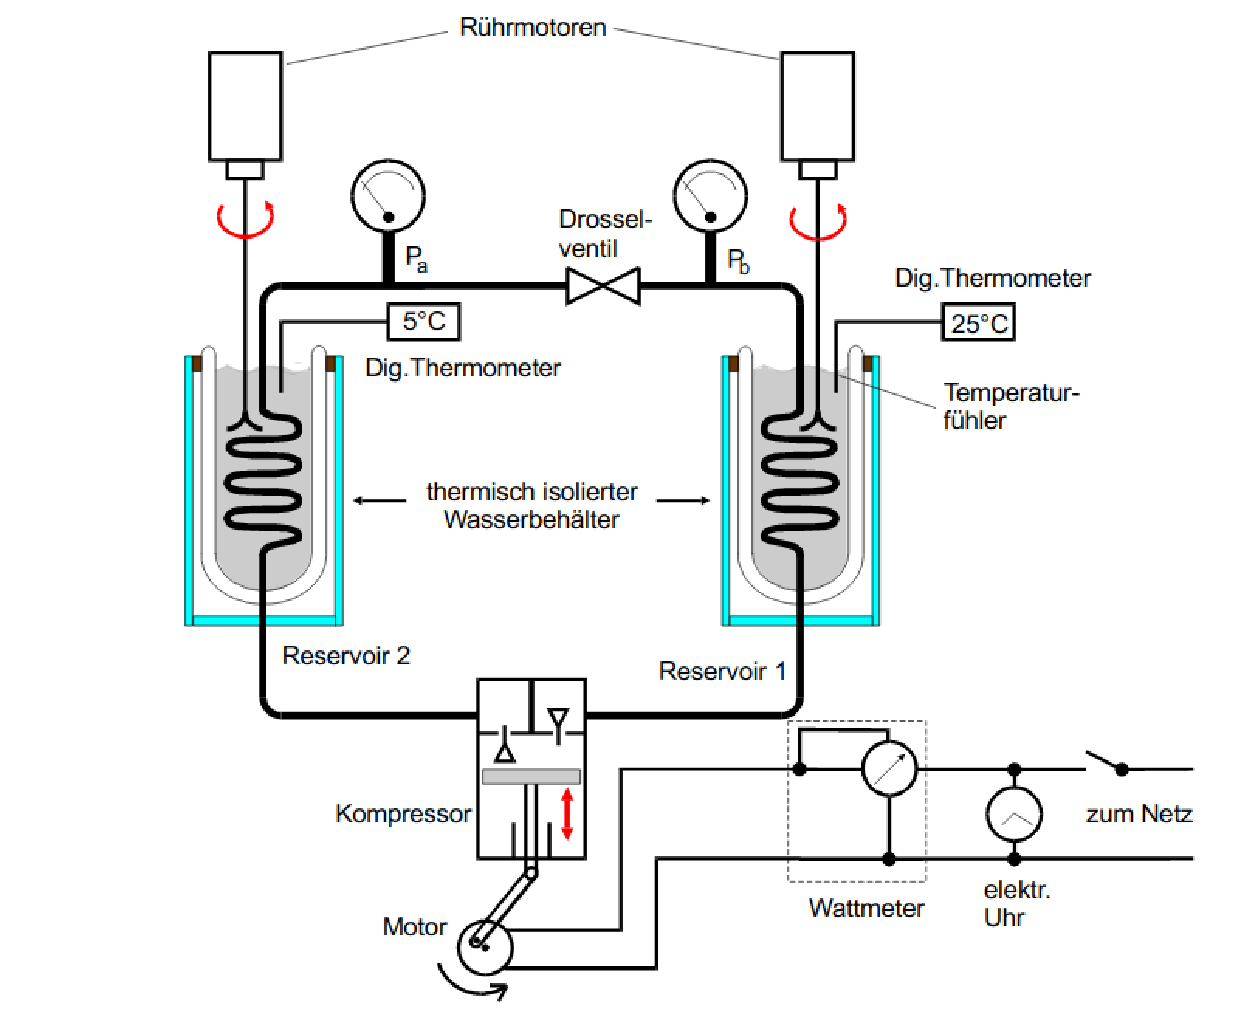
\includegraphics{Darstellung_Waermepumpe.pdf}
\caption{Schematische Darstellung der Messapparatur \cite[4]{anleitung}}
\end{figure}
Die Reservoire bestehen aus thermisch isolierten Eimern, sodass die Wassertemperatur nicht von der Umgebungstemperatur beeinflusst wird.

Zu Beginn des Experimentes werden in beide Eimer \SI{4}{\litre} kaltes Wasser gefüllt. 
Mit Rührmotoren wird das Wasser in den Eimern gerührt, damit dessen Temperatur einheitlich ist.
Nachdem die Anfangswerte notiert wurden und der Netzschalter des Kompressors umgelegt, wird im Minutentakt die Temperatur des Reservoirs 1 $T_{1}$, die Drücke $p_{\text{b}}$ und $p_{\text{a}}$, die Temperatur des Reservoirs 2 $T_{2}$ und die Leistungsaufnahme des Kompressors $N$.
Die Messung wird abgebrochen, sobald $T_1$ den Wert von \SI{50}{\celsius} erreicht hat.

